\subsection{3D-Tetris Environment}

This code is modified from the code of the 2D-Tetris environment.

\paragraph{Board and block.}
In our setting, the board is set to be \(4 \times 4 \times 20\), where \(20\) is the vertical height. The 3D environment contains four types of blocks, as illustrated in Figure~\ref{fig:4Blocks}. Each block can rotate freely in 90-degree increments along the three spatial axes. We precompute and store all unique rotational variants for each block shape. A block may be placed in any position on the board as long as it does not exceed the boundary or collide with existing blocks.

\paragraph{Action space.}
An action is defined as a tuple \((r, x, y)\), where \(r\) indexes a valid rotation of the current block, and \((x, y)\) indicates the horizontal position. For each piece, we enumerate all legal actions across its precomputed rotations and all valid horizontal placements. Once an action is selected, the block is dropped vertically until it reaches the lowest feasible height.

\paragraph{State space.}
The full state consists of the current 3D board configuration and the falling block. To support learning algorithms, we represent the state after each action with a 4-dimensional feature vector \(s = \ell, h, b, H\), where:
\begin{itemize}
    \item \(\ell\) is the number of fully filled horizontal planes, which will be cleared in the Tetris game,
    \item \(h\) counts the empty cells beneath filled blocks in each column,
    \item \(b\) measures the height differences between neighboring columns, and
    \item \(H\) is the total sum of column heights across the board.
\end{itemize}
This abstract representation captures key spatial features relevant to gameplay and is useful for reinforcement learning agents.

\paragraph{Environment mechanic.}
At each step, the agent selects one of the legal actions to place the current block. The block is inserted into the board at the lowest possible height, determined by gravity and the existing filled cells. After placement, the environment checks for any completely filled horizontal planes. If such planes exist, they are cleared, and all blocks above them are shifted downward to fill the empty space. The environment then randomly selects the next block and its orientation. The reward given after each action increases polynomially with the number of planes cleared, encouraging the agent to complete multiple planes simultaneously.

\subsection{Deep Q Learning for 3D-Tetris}
We train a Deep Q-Network (DQN) agent to play the 3D-Tetris game described previously. Unlike the standard DQN, which operates over a fixed discrete action space, our agent dynamically enumerates valid actions at each step based on the current block's shape, orientation, and available board positions. This design accommodates the geometry-dependent nature of legal moves in 3D-Tetris. The overall workflow of the training process is visualized in Figure~\ref{fig:Workflow}.

\paragraph{Q-network.}
The Q-network is a fully connected neural network that takes a 4-dimensional state feature vector as input and outputs a scalar Q-value. Since the number of legal actions changes with each board state, the network evaluates Q-values independently for each possible next state produced by enumerating valid actions. This enables flexible decision-making without assuming a fixed-size action space.

\paragraph{Training process.}
At each step, the agent enumerates all legal actions and corresponding next states. It then uses an $\epsilon$-greedy policy to either select an action randomly or choose the one with the highest predicted Q-value. The resulting transition $(s, r, s', \text{done})$ is stored in a replay buffer. If the game ends, the environment resets for a new episode.

\begin{figure}
    \centering
    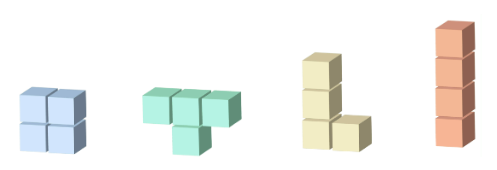
\includegraphics[width=0.5\linewidth]{4Blocks.png}
    \caption{Four types of blocks in 3D-Tetris}
    \label{fig:4Blocks}
\end{figure}

\begin{figure}
    \centering
    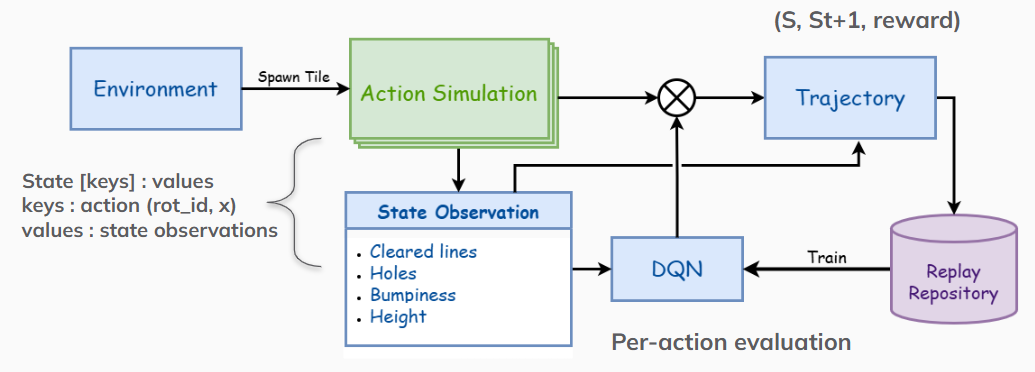
\includegraphics[width=0.75\linewidth]{Work-flow.png}
    \caption{Training process of the DQN}
    \label{fig:Workflow}
\end{figure}
